\newcommand{\institute}{Sprach- und literaturwissenschaftliche Fakultät}
\newcommand{\department}{Institut für Anglistik und Amerikanistik}
\newcommand{\university}{Humboldt-Universität zu Berlin}
\newcommand{\researchGroup}{Databases and Information Systems}
\newcommand{\city}{Berlin}
\newcommand{\country}{Deutschland}
%%%%%%%%% Begin Titlepage %%%%%%%%%%%
\begin{titlepage}
  %\thispagestyle{empty}%
  %  \begin{picture}(2,0)(0,-1.35)
  %  \includegraphics[height=\logosize]{images/agdb_logo}
  %\end{picture}\hfill
  %\begin{picture}(4,0)(1.6,-1.35)
  %  \includegraphics[height=\logosize]{images/fu_logo}
  %\end{picture}\vskip0pt
  \vspace*{-1.1cm}%
  \hskip-\dimexpr\abstand+\randI\relax%
  \colorbox{HUpantone}{%
  \begin{minipage}[t]%[2\abstand][c]
  	{\paperwidth}%
    \vspace{2ex}
    \hskip\dimexpr\abstand+\randI\relax%
      \begin{minipage}{\dimexpr\paperwidth-\randA-\randI\relax}
      \color{white}%
      \Large\thetitle
      \end{minipage}
    \vspace{2ex}
  \end{minipage}%
  }\vskip-8.5pt
  \hskip-\dimexpr\abstand+\randI\relax%
  \colorbox{lightgray}{%
  \begin{minipage}[t][1cm][c]{\paperwidth}
    \hskip\dimexpr\abstand+\randI\relax%
    \textit{\textbf{Bachelorarbeit} zur Erlangung des akademischen Grades} \par
    \hskip\dimexpr\abstand+\randI\relax%
    \textbf{\textit{\degree}} \textit{im Fach \textbf{Englisch}}.
  \end{minipage}}\vfill%\vspace{5\baselineskip}
  
%%%%%%%%%%% datas %%%%%%%%%%%
    Humboldt-Universität zu Berlin \par
    Sprach- und literaturwissenschaftliche Fakultät \par
    Institut für Anglistik und Amerikanistik \par
    \vspace{2\baselineskip}
    eingereicht von \par
    \textbf{\theauthor} \par
    geb. am 23.06.1997 \par
    in Stawropol, Russische Föderation \par
    \vfill%vspace{5\baselineskip}

	% 1. ADVISOR
    \textbf{\underline{Gutachter*innen:}}\par
    \textbf{\fstAdvisor}%
      \footnote{\fstAdvisorsDepartment,
      \fstAdvisorsAG},
    \fstAdvisorsUniversity,
      \fstAdvisorsCountry\par
    % 2. ADVISOR
    \textbf{\sndAdvisor}%
      \footnote{\sndAdvisorsDepartment,
      \sndAdvisorsAG},
      \sndAdvisorsUniversity,
      \fstAdvisorsCountry
   	\par\vspace{3.5\baselineskip}
    
    \textbf{\underline{Zitat:}}\par 
    \textbf{Bondarenko, Daniil}.
    (\Year).
    \textit{\thetitle}. 
    \university, \thesisKind{} Thesis. \par
    \vspace{2.5\baselineskip}
    
    \textbf{Version:} \versionnumber \par
    \vspace{0.5\baselineskip}
    Berlin, den \thedate\par
    \vfill
\end{titlepage}

\thispagestyle{empty} % no page number
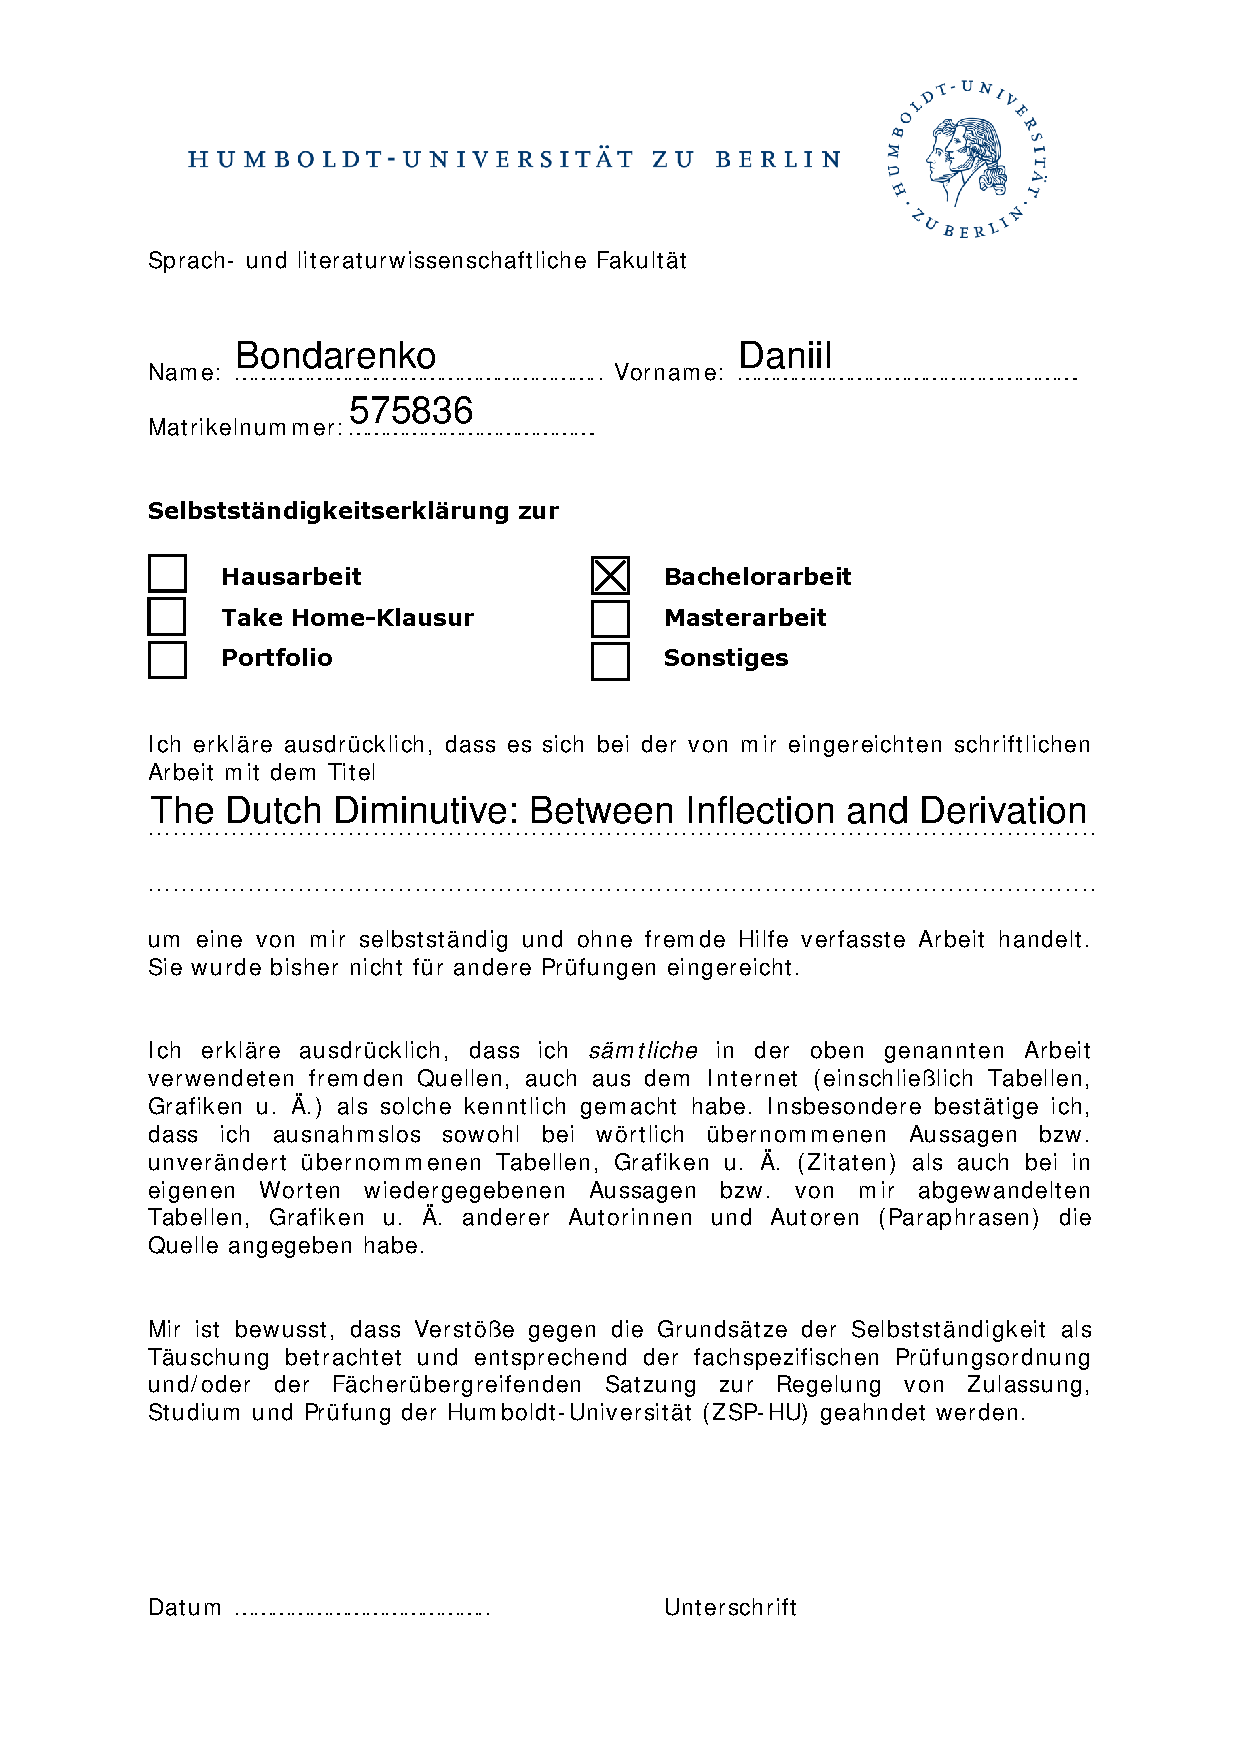
\includepdf{images/selbststaendigkeitserklaerung_2021.pdf}


\thispagestyle{empty} % no page number
\setcounter{page}{1}
\vspace*{3cm}
\begin{center}
\begin{minipage}[c]{0.6\paperwidth}%
    \vspace{2ex}
    \textit{En de vogels vliegen van West naar Oost Berlijn} \\
    \textit{Worden niet teruggefloten, ook niet neergeschoten} \\
    \textit{Over de muur, over het ijzeren gordijn} \\
    \textit{Omdat ze soms in het oosten, soms ook in het westen willen zijn} \\
    \textit{Omdat er brood ligt soms bij de Gedächtniskirche} \\
    \textit{Soms op het Alexanderplein.} \par
    \vspace{2ex}
    \hfill -- Klein Orkest, 1984
  \end{minipage}
\end{center}